%File: formatting-instructions-latex-2023.tex
%release 2023.0
\documentclass[letterpaper]{article} % DO NOT CHANGE THIS
\usepackage{aaai23}  % DO NOT CHANGE THIS
\usepackage{times}  % DO NOT CHANGE THIS
\usepackage{helvet}  % DO NOT CHANGE THIS
\usepackage{courier}  % DO NOT CHANGE THIS
\usepackage[hyphens]{url}  % DO NOT CHANGE THIS
\usepackage{graphicx} % DO NOT CHANGE THIS
\urlstyle{rm} % DO NOT CHANGE THIS
\def\UrlFont{\rm}  % DO NOT CHANGE THIS
\usepackage{natbib}  % DO NOT CHANGE THIS AND DO NOT ADD ANY OPTIONS TO IT
\usepackage{caption} % DO NOT CHANGE THIS AND DO NOT ADD ANY OPTIONS TO IT
\frenchspacing  % DO NOT CHANGE THIS
\setlength{\pdfpagewidth}{8.5in}  % DO NOT CHANGE THIS
\setlength{\pdfpageheight}{11in}  % DO NOT CHANGE THIS
%
% These are recommended to typeset algorithms but not required. See the subsubsection on algorithms. Remove them if you don't have algorithms in your paper.
\usepackage{algorithm}
% \usepackage{algorithmic}

%
% These are are recommended to typeset listings but not required. See the subsubsection on listing. Remove this block if you don't have listings in your paper.
\usepackage{newfloat}
\usepackage{listings}
\DeclareCaptionStyle{ruled}{labelfont=normalfont,labelsep=colon,strut=off} % DO NOT CHANGE THIS
\lstset{%
	basicstyle={\footnotesize\ttfamily},% footnotesize acceptable for monospace
	numbers=left,numberstyle=\footnotesize,xleftmargin=2em,% show line numbers, remove this entire line if you don't want the numbers.
	aboveskip=0pt,belowskip=0pt,%
	showstringspaces=false,tabsize=2,breaklines=true}
\floatstyle{ruled}
\newfloat{listing}{tb}{lst}{}
\floatname{listing}{Listing}
%
% Keep the \pdfinfo as shown here. There's no need
% for you to add the /Title and /Author tags.




\usepackage{booktabs}
\usepackage{amssymb}
\usepackage{amsmath,bm}
\usepackage{multirow}







% DISALLOWED PACKAGES
% \usepackage{authblk} -- This package is specifically forbidden
% \usepackage{balance} -- This package is specifically forbidden
% \usepackage{color (if used in text)
% \usepackage{CJK} -- This package is specifically forbidden
% \usepackage{float} -- This package is specifically forbidden
% \usepackage{flushend} -- This package is specifically forbidden
% \usepackage{fontenc} -- This package is specifically forbidden
% \usepackage{fullpage} -- This package is specifically forbidden
% \usepackage{geometry} -- This package is specifically forbidden
% \usepackage{grffile} -- This package is specifically forbidden
% \usepackage{hyperref} -- This package is specifically forbidden
% \usepackage{navigator} -- This package is specifically forbidden
% (or any other package that embeds links such as navigator or hyperref)
% \indentfirst} -- This package is specifically forbidden
% \layout} -- This package is specifically forbidden
% \multicol} -- This package is specifically forbidden
% \nameref} -- This package is specifically forbidden
% \usepackage{savetrees} -- This package is specifically forbidden
% \usepackage{setspace} -- This package is specifically forbidden
% \usepackage{stfloats} -- This package is specifically forbidden
% \usepackage{tabu} -- This package is specifically forbidden
% \usepackage{titlesec} -- This package is specifically forbidden
% \usepackage{tocbibind} -- This package is specifically forbidden
% \usepackage{ulem} -- This package is specifically forbidden
% \usepackage{wrapfig} -- This package is specifically forbidden
% DISALLOWED COMMANDS
\nocopyright
% -- Your paper will not be published if you use this command
% \addtolength -- This command may not be used
% \balance -- This command may not be used
% \baselinestretch -- Your paper will not be published if you use this command
%  -- No page breaks of any kind may be used for the final version of your paper
% \columnsep -- This command may not be used
%  -- No page breaks of any kind may be used for the final version of your paper
% \pagebreak -- No page breaks of any kind may be used for the final version of your paperr
% \pagestyle -- This command may not be used
% \tiny -- This is not an acceptable font size.
% \vspace{- -- No negative value may be used in proximity of a caption, figure, table, section, subsection, subsubsection, or reference
% \vskip{- -- No negative value may be used to alter spacing above or below a caption, figure, table, section, subsection, subsubsection, or reference

\setcounter{secnumdepth}{0} %May be changed to 1 or 2 if section numbers are desired.

% The file aaai23.sty is the style file for AAAI Press
% proceedings, working notes, and technical reports.
%

% Title

% Your title must be in mixed case, not sentence case.
% That means all verbs (including short verbs like be, is, using,and go),
% nouns, adverbs, adjectives should be capitalized, including both words in hyphenated terms, while
% articles, conjunctions, and prepositions are lower case unless they
% directly follow a colon or long dash
% \title{AAAI Press Formatting Instructions \\for Authors Using \LaTeX{} --- A Guide}
% \author{
%     %Authors
%     % All authors must be in the same font size and format.
%     Written by AAAI Press Staff\textsuperscript{\rm 1}\thanks{With help from the AAAI Publications Committee.}\\
%     AAAI Style Contributions by Pater Patel Schneider,
%     Sunil Issar,\\
%     J. Scott Penberthy,
%     George Ferguson,
%     Hans Guesgen,
%     Francisco Cruz\equalcontrib,
%     Marc Pujol-Gonzalez\equalcontrib
% }
% \affiliations{
%     %Afiliations
%     \textsuperscript{\rm 1}Association for the Advancement of Artificial Intelligence\\
%     % If you have multiple authors and multiple affiliations
%     % use superscripts in text and roman font to identify them.
%     % For example,

%     % Sunil Issar, \textsuperscript{\rm 2}
%     % J. Scott Penberthy, \textsuperscript{\rm 3}
%     % George Ferguson,\textsuperscript{\rm 4}
%     % Hans Guesgen, \textsuperscript{\rm 5}.
%     % Note that the comma should be placed BEFORE the superscript for optimum readability

%     1900 Embarcadero Road, Suite 101\\
%     Palo Alto, California 94303-3310 USA\\
%     % email address must be in roman text type, not monospace or sans serif
%     publications23@aaai.org
% %
% % See more examples next
% }

%Example, Single Author, ->> remove \iffalse,\fi and place them surrounding AAAI title to use it
\iffalse
\title{My Publication Title --- Single Author}
\author {
    Author Name
}
\affiliations{
    Affiliation\\
    Affiliation Line 2\\
    name@example.com
}
\fi

% \iffalse
%Example, Multiple Authors, ->> remove \iffalse,\fi and place them surrounding AAAI title to use it
\title{Bi-directional Feature Reconstruction Network for Fine-Grained \\ Few-Shot Image Classification}
\author {
    % Authors
    Jijie Wu\textsuperscript{\rm 1},
    Dongliang Chang\textsuperscript{\rm 2},
    Aneeshan Sain\textsuperscript{\rm 3},\\
    Xiaoxu Li\textsuperscript{\rm 1}\thanks{indicates corresponding author.},
    Zhanyu Ma\textsuperscript{\rm 2},
    Jie Cao\textsuperscript{\rm 1},
    Jun Guo\textsuperscript{\rm 2},
    and Yi-Zhe Song\textsuperscript{\rm 3}
}
\affiliations {
    % Affiliations
    \textsuperscript{\rm 1}School of Computer and Communications, Lanzhou University of Technology, Lanzhou, China\\
    \textsuperscript{\rm 2}School of Artificial Intelligence, Beijing University of Posts and Telecommunications, Beijing, China\\
    \textsuperscript{\rm 3}SketchX, CVSSP, University of Surrey, United Kingdom \\

    \{jijie, lixiaoxu, caoj\}@lut.edu.cn,
    \{changdongliang, mazhanyu, guojun\}@bupt.edu.cn,
    \{a.sain, y.song\}@surrey.ac.uk
}
% \fi


% REMOVE THIS: bibentry
% This is only needed to show inline citations in the guidelines document. You should not need it and can safely delete it.
% \usepackage{bibentry}
% END REMOVE bibentry

\begin{document}

\maketitle

\begin{abstract}
The main challenge for fine-grained few-shot image classification is to learn feature representations with higher inter-class and lower intra-class variations, with a mere few labelled samples. Conventional few-shot learning methods however cannot be naively adopted for this fine-grained setting -- a quick pilot study reveals that they in fact push for the opposite (i.e., lower inter-class variations and higher intra-class variations). To alleviate this problem, prior works predominately use a support set to reconstruct the query image and then utilize metric learning to determine its category. Upon careful inspection, we further reveal that such unidirectional reconstruction methods only help to increase inter-class variations and are not effective in tackling intra-class variations. In this paper, we for the first time introduce a bi-reconstruction mechanism that can simultaneously accommodate for inter-class and intra-class variations. In addition to using the support set to reconstruct the query set for increasing inter-class variations, we further use the query set to reconstruct the support set for reducing intra-class variations. This design effectively helps the model to explore more subtle and discriminative features which is key for the fine-grained problem in hand. Furthermore, we also construct a self-reconstruction module to work alongside the bi-directional module to make the features even more discriminative. Experimental results on three widely used fine-grained image classification datasets consistently show considerable improvements compared with other methods.
Codes are available at: https://github.com/PRIS-CV/Bi-FRN.
\end{abstract}

\section{Introduction}

\begin{figure}[!htp]
  \centering
  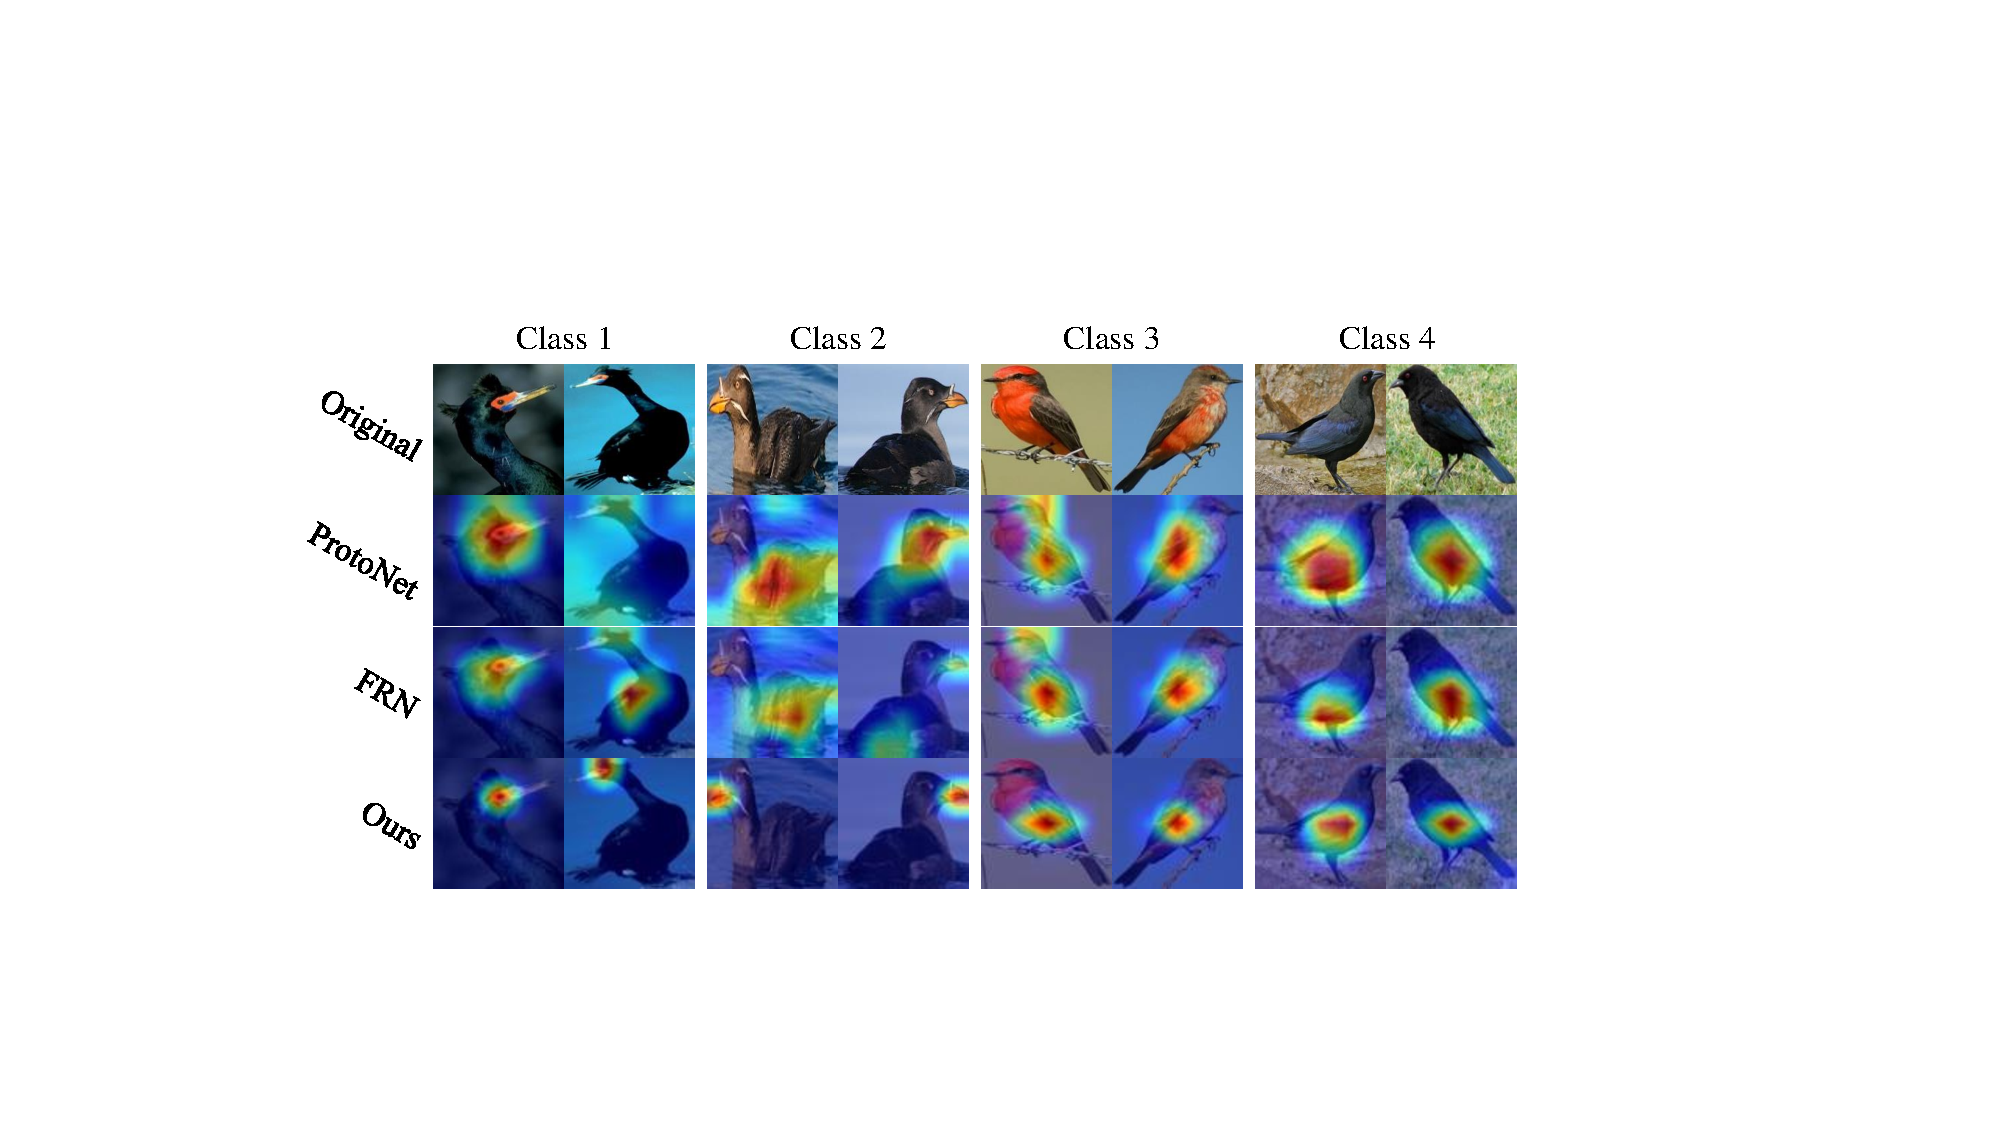
\includegraphics[width=0.85\linewidth]{figures/1.1.pdf}
  \caption{Visualization of the localized regions returned from Eigen-CAM~\cite{muhammad2020eigen} based on a ProtoNet~\cite{NIPS2017_cb8da676} model (trained on CUB-200-211 dataset) optimized by the traditional method, the FRN~\cite{Wertheimer_2021_CVPR}, and the proposed method. The higher energy region denotes the more discriminative part in the image.}
  \label{fig:1}
\end{figure}



Few-shot fine-grained image classification~\cite{Huang2021LowRankPA,9293172} has emerged very recently as an important means to tackle the data scarcity problem widely facing fine-grained analysis~\cite{3401454f29a841a29142c97833857e78}. As per the conventional few-shot setting, it asks for effective model transfer given just a few support samples. The differences however lies in the unique characteristics brought by the fine-grained nature of the problem -- the model needs to focus on learning subtle and discriminative features to discriminate not only on the category level (as per conventional few-shot), but importantly also on intra-class level differentiating fine-grained visual differences amongst class instances.

It is therefore not surprising that traditional few-shot methods, when applied to the {fine-grained} problem, can no longer hold their promises. This is clearly seen in Figure~\ref{fig:1}, where we apply ProtoNet~\cite{NIPS2017_cb8da676} on the ``birds'' dataset~\cite{WelinderEtal2010} -- the model {tends to encourage} lower inter-class variations and higher intra-class variations, which is the very opposite of our goal of fine-grained image classification.



Attempts have been made on adapting traditional few-shot learning methods to the fine-grained scenario. Early attempts~\cite{Huang2021LowRankPA, sun2020few, zhu2020multi} have however focused on devising complex architectural designs which resulted in marginal gains over their vanilla counterparts. It was not until very recently that reconstruction-based methods have gained popularity~\cite{Wertheimer_2021_CVPR, NEURIPS2020_fa28c6cd} and consequently achieved state-of-the art performance. Through specifically engineering for {support-query} feature alignment, they naturally encourage fine-grained transfer. Effects of this can be observed in Figure \ref{fig:1}, where feature regions learned by FRN~\cite{Wertheimer_2021_CVPR} tend to be more fine-grained when compared with ProtoNet~\cite{NIPS2017_cb8da676}.


\begin{figure*}[ht]
  \centering
  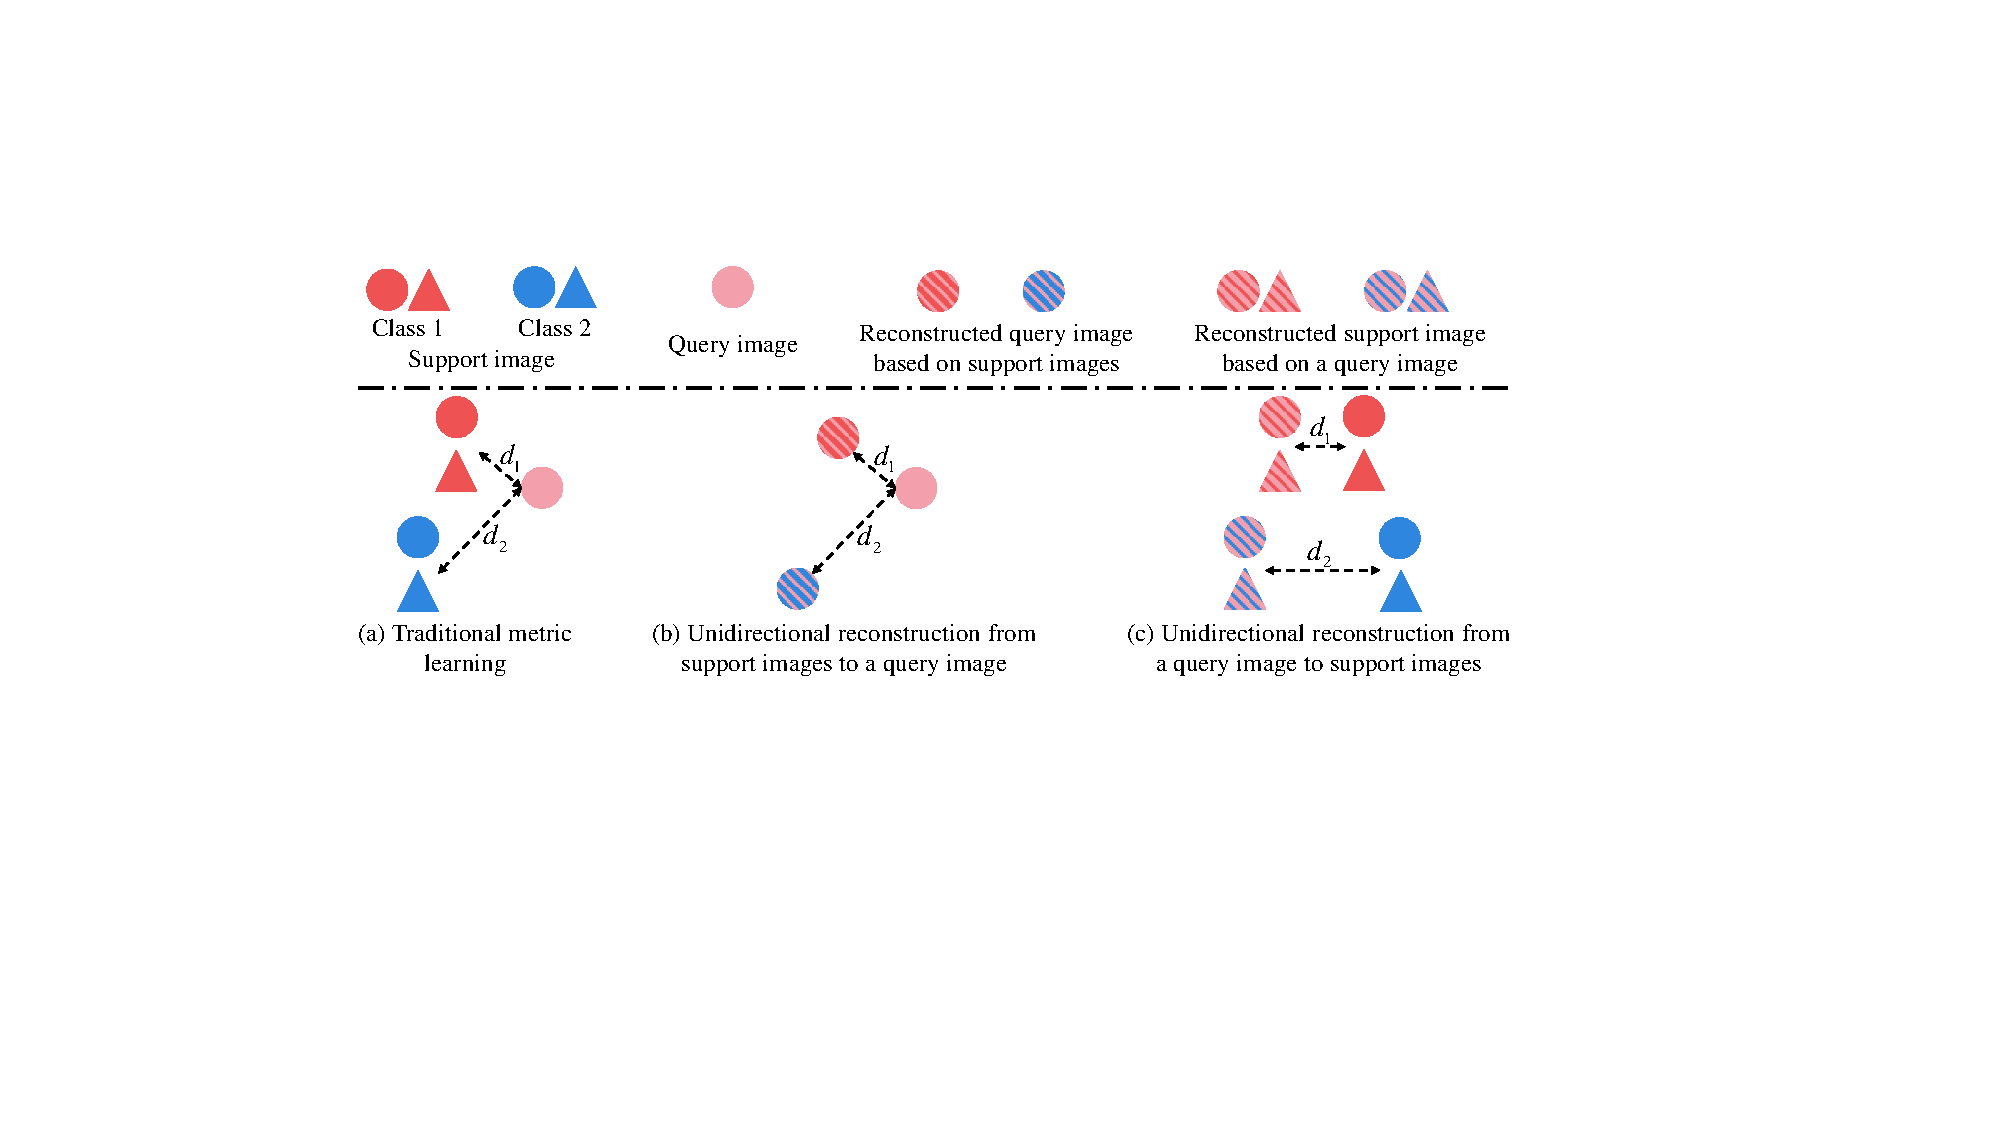
\includegraphics[width=0.8\linewidth]{figures/1.2.pdf}
  \caption{(a) is the traditional metric based method. (b) is the method proposed in~\cite{Wertheimer_2021_CVPR}. (b) + (c) is the method proposed in this paper. (b) can help the model increase the inter-class variations, and (c) can help the model decrease the intra-class variations.}
  \label{fig:1.2}
\end{figure*}


However upon careful inspection, we importantly observe that although the model can focus on more subtle and discriminative regions, the semantic information they represented is nonetheless disparate between any two samples belonging to the same class (e.g., ``Class 1'' FRN focused on different parts of a bird). This seems to suggest that these reconstruction-based methods still suffer from having large intra-class variations, which is counter-productive for overall fine-grained learning (large inter-class variations and small intra-class variations). In other words, such methods only help to increase inter-class variations and do not reduce intra-class variations very well. The reason, we conjecture, is that the existing reconstruction-based methods~\cite{Wertheimer_2021_CVPR, NEURIPS2020_fa28c6cd} (as shown in Figure~\ref{fig:1.2}(b)) works in a unidirectional fashion, i.e., reconstruction only happens one way from support features to query features.
Consequently, it can only constrain the relationship between reconstructed query features and original query features to increase inter-class variations. This however fails to constrain the relationship between samples within each class in the support set, which is pivotal in decreasing intra-class variations.




As such, in this paper, we for the first time introduce a bi-directional reconstruction mechanism for few-shot fine-grained classification. Instead of using the support set to reconstruct the query set to increase inter-class variations only (as shown in Figure~\ref{fig:1.2}(b)),
we additionally use the query set to reconstruct the support set to simultaneously reduce intra-class variations (as shown in Figure~\ref{fig:1.2}(c)). This modification might sound overly simple at first sight, it however importantly fulfills both desired learning outcomes for the fine-grained setting -- support to query to encourage large inter-class variations, and query to support to encourage small intra-class variations
(see Section \ref{Ablation} for a detailed explanation).


Our bi-directional feature reconstruction framework mainly contains four modules: (i) a feature extraction module, (ii) a self-reconstruction module, (iii) a mutual bi-directional reconstruction module, and (iv) a distance metric module. (i) and (iv) are common to a reconstruction-based approach~\cite{Wertheimer_2021_CVPR}. In addition to the proposed bi-directional module (iii), we also find use of a self-reconstruction module (ii) to benefit fine-grained feature learning, and works well with the former in terms of increasing inter-class variations and reducing intra-class variations. Ablative studies in Section \ref{Ablation} show both to be effective {and indispensable} for few-shot fine-grained learning.

%, where bi-directional reconstruction \textit{alone} plays a major role (beating state-of-the-art classification performance by 4\%), and self-reconstruction further boosts performance by 6\%.


In summary, our contributions are three-fold:
1) We reveal the key problem in current reconstruction-based few-shot fine-grained classification lies with its inability in minimising intra-class variations.
2) We for the first time propose a bi-directional reconstruction network that simultaneously increase inter-class variations while reducing intra-class variations by way of a mutual {support-query and query-support} reconstruction.
3) Experimental results and ablative analyses on three fine-grained few-shot image datasets consistently demonstrate the superiority of the proposed method and reveal insights on why the bi-directional approach is effective.




\section{Related works}



\textbf{Metric-Based Few-shot Learning:}
In few-shot learning methods, metric-based methods have received extensive attention owing to their simplicity and efficiency~\cite{Li2021DeepML}.
{A plethora of earlier works have adopted fixed metric or learnable module to learn a good metric embedding~\cite{NIPS2017_cb8da676, DBLP:conf/nips/VinyalsBLKW16, 8578229}. These methods classify samples according to distance or similarity.}
Recently, GNN-based few-shot methods~\cite{garcia2018fewshot, Kim_2019_CVPR, Yang_2020_CVPR} adopted graph neural networks (GNN) to model the similarity measurement -- their advantage being that samples have a rich relational structure.
In addition to these classic ones, some metric-based methods for fine-grained image classification have also emerged.
While DN4~\cite{8953758} proposed a local descriptor-based image-to-class measure, using local features of samples to learn feature metric, {BSNet~\cite{9293172} used a bi-similarity network to learn fewer but more discriminative regions using a combination of two different metrics.}
NDPNet~\cite{Zhang2021NDPNetAN} designed a feature re-abstraction embedding network that projects the local features into the proposed similarity metric learning network to learn discriminative projection factors.
Our method adopts a fixed euclidean distance to measure the error between construction features and origin features.




\textbf{Alignment-based Few-shot Learning:}
Alignment-based fine-grained few-shot methods pay more attention to align the spatial positions of objects in images and then classify them based on a similarity measure.
Unlike PARN~\cite{Wu_2019_ICCV} which is a position-aware relational network that aligns similar objects in spatial position and learns more flexible and robust metric capabilities,
Semantic Alignment Metric Learning (SAML)~\cite{Hao2019CollectAS} aligns the semantically relevant dominant objects in fine-grained images using a collect-and-select strategy.
DeepEMD~\cite{Zhang_2020_CVPR} uses the Earth Mover's Distance to generate the optimal matching flows between two local feature sets and computes the distance between two images based on the optimal matching flows and matching costs.
In addition to these alignment-based methods above, reconstruction-based methods are also good for aligning spatial positions of objects from different fine-grained images.
CTX~\cite{NEURIPS2020_fa28c6cd} constructs a novel transformer-based neural network, which can find a coarse spatial relationship between the query and the labelled images, and then compute the distances between spatially-corresponding features to predict the label of samples.
Alleviating the need for any new modules or large-scale learnable parameters FRN~\cite{Wertheimer_2021_CVPR} obtains the optimal reconstruction weights in the closed form solution to reconstruct query features from support features.
Unlike these existing reconstruction based methods, we introduce bi-directional reconstruction method, that not only reconstructs query samples based on support samples for increasing the inter-class variations, but also reconstructs support samples based on a query sample for reducing the intra-class variations.



% \acmISBN{}

\textbf{Attention Mechanism:}
Vaswani et al.~\cite{NIPS2017_3f5ee243} first proposed the self-attention mechanism and then used it to built a new simple network architecture, namely Transformer.
Besides achieving success in natural language processing~\cite{NIPS2017_3f5ee243, Devlin2019BERTPO, brown2020language}, this architecture also works well in computer vision tasks~\cite{dosovitskiy2021an, hassani2021escaping, Chen2021CrossViTCM}.
Recently, some few-shot learning works have gradually begun to adopt the self-attention mechanism. Han-Jia Ye et al.~\cite{Ye_2020_CVPR} proposed a Few-shot Embedding Adaptation with Transformer (FEAT) for few-shot learning. Here authors constructed set-to-set functions using a variety of approximators and found Transformer to be the most efficient option that {can model interactions between images in a set and hence enable co-adaptation of each image.}
{Unlike FEAT where the transformer structure is only used for support samples, CTX~\cite{NEURIPS2020_fa28c6cd} uses self-attention to calculate the spatial attention weights of query sample and support samples and learn a query-aligned class prototype. It then calculates the distance between the query sample and the aligned class prototype to classify the query sample.}
The proposed few-shot classification method also introduced the self-attention mechanism adopted in the transformer to learn optimal reconstruction weights in our self-reconstruction module and mutual reconstruction module.



\section{Methodology}
In this section, we describe our proposed method, starting with a formulation of the proposed method followed by an overview and an in-depth description of each component.





\subsection{The Problem Formulation}
Given a dataset $D = \{(x_i,y_i), y_i \in Y\}$, we divide it into three parts, that is, $D_{base} = \{(x_i,y_i), y_i \in Y_{base}\}$, $D_{val} = \{(x_i,y_i), y_i \in Y_{val}\}$ and $D_{novel} =\{ (x_i,y_i), y_i \in Y_{novel}\}$, where $x_i$ and  $y_i$ are the original feature vector and class label of the $i^\text{th}$ image, respectively.
The categories of these three parts are disjoint, i.e., $Y_{base} \cap Y_{val} \cap Y_{novel} = \varnothing$, and $Y_{base} \cup Y_{val} \cup Y_{novel} = Y$.
Few-shot classification aims to improve a $C$-way $K$-shot classification performance on $D_{novel}$ by learning knowledge from $D_{base}$ and $D_{val}$.
% In $C$-way $K$-shot classification, it usually contains lots of tasks.
For such a task, there are $C$ classes sampled randomly from $D_{novel}$, and each class only has $K$ {randomly sampled} labelled (support) samples $S$, and $M$ {randomly sampled} unlabelled (query) samples $Q$.


Many few-shot methods adopt the meta-learning paradigm~\cite{Finn2017ModelAgnosticMF, ye2022how}. Specifically, the training process of these methods on $D_{base}$ is the same as the prediction process on $D_{novel}$. Their purpose is to learn the meta-knowledge of learning a category concept based on a few labelled samples.
In the meta-training phase, the few-shot classification model learns the categories of query samples based on few support samples in each task on $D_{base}$. The optimal model is selected by evaluating performance of the {few-shot classification model} on multiple tasks on $D_{val}$. In meta-test phase, the final performance of the optimal model are commonly evaluated by the average accuracy on all sampled tasks of $D_{novel}$.

\subsection{Overview}

\begin{figure*}[!ht]
  \centering
  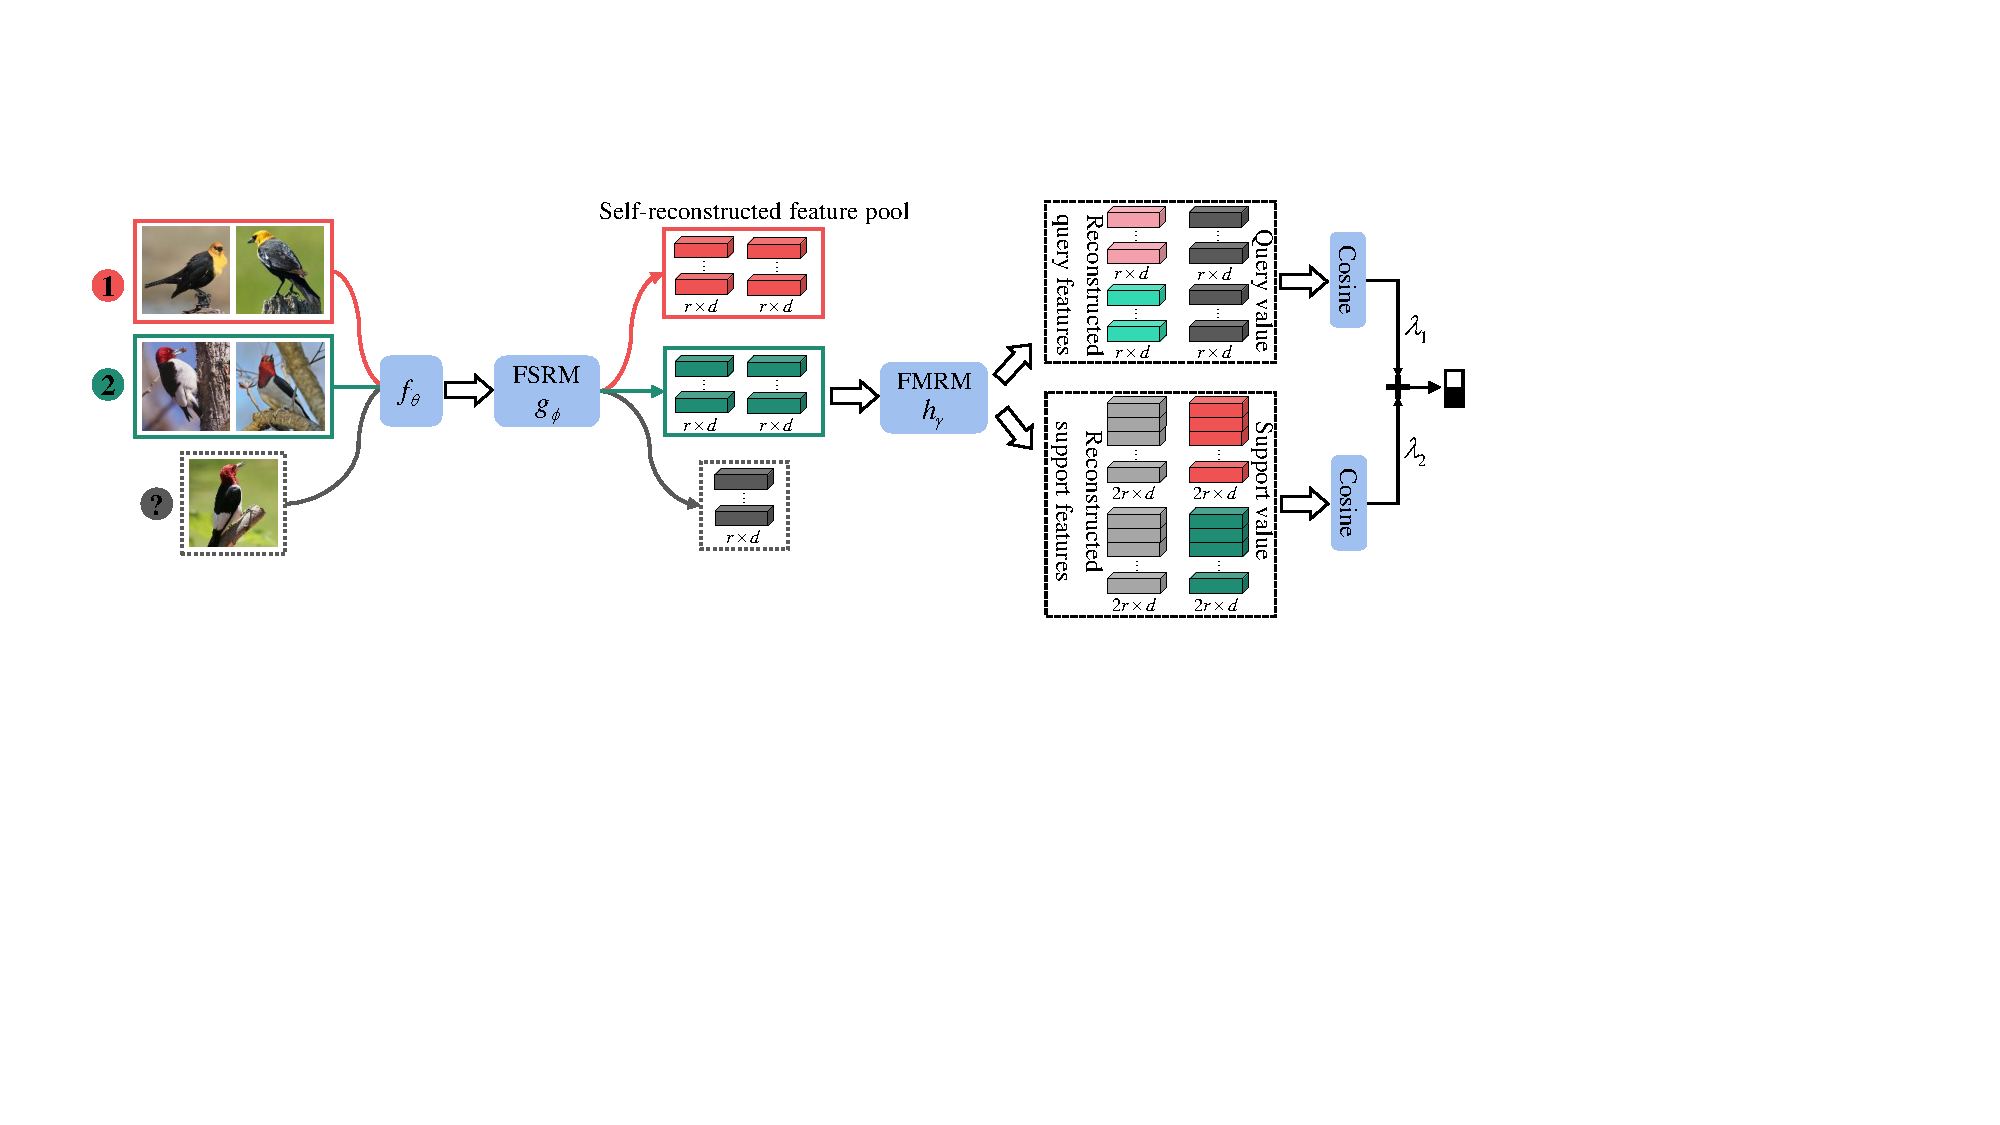
\includegraphics[width=0.9\linewidth]{figures/3.1.pdf}
  \caption{The proposed Bi-Directional feature reconstruction network. FSRM refers to Feature Self-reconstruction Module and FMRM refers to Feature Mutual Reconstruction Module.}
  \label{fig:3.1}
\end{figure*}

Learning subtle and discriminative features is crucial for fine-grained few-shot image classification. Considering that the existing reconstruction-based methods, which mostly reconstruct query features based on support features, fail to reduce intra-class variations adequately, we propose a  bi-directional reconstruction network.


As shown in Figure~\ref{fig:3.1}, our model consists of four modules:
the first is embedding module $f_{\theta}$ for extracting deep convolutional image features. This can be a traditional convolutional neural network or a residual network.
The second is a feature self-reconstruction module $g_{\phi}$, in which the convolutional features of each image are reconstructed by themselves based on a self-attention mechanism.
This module can make the similar local features become more similar, while dissimilar ones even more dissimilar, and additionally benefits the following feature mutual reconstruction.
The third is a feature mutual reconstruction module, $h_{\gamma}$, which reconstructs sample features in a bidirectional form. This module not only uses the support sample to reconstruct the query sample but also reconstructs the support sample from the query sample. Compared with the existing unidirectional reconstruction which only focuses on increasing inter-class variations of features, the bi-directional reconstruction adds another function -- reducing the intra-class variations of features.
% \textcolor{red}{An in-depth analysis about the feature mutual reconstruction can be found in the supplementary material.}
Finally, the fourth is a {Euclidean} metric module, which is in charge of calculating the distance between query sample and reconstructed query sample, as well as support samples and reconstructed support samples. The weighted sum of the two distances are used for classifying query samples.





\subsection{Feature Self-Reconstruction Module (FSRM)}





\begin{figure}[htp]
\centering
  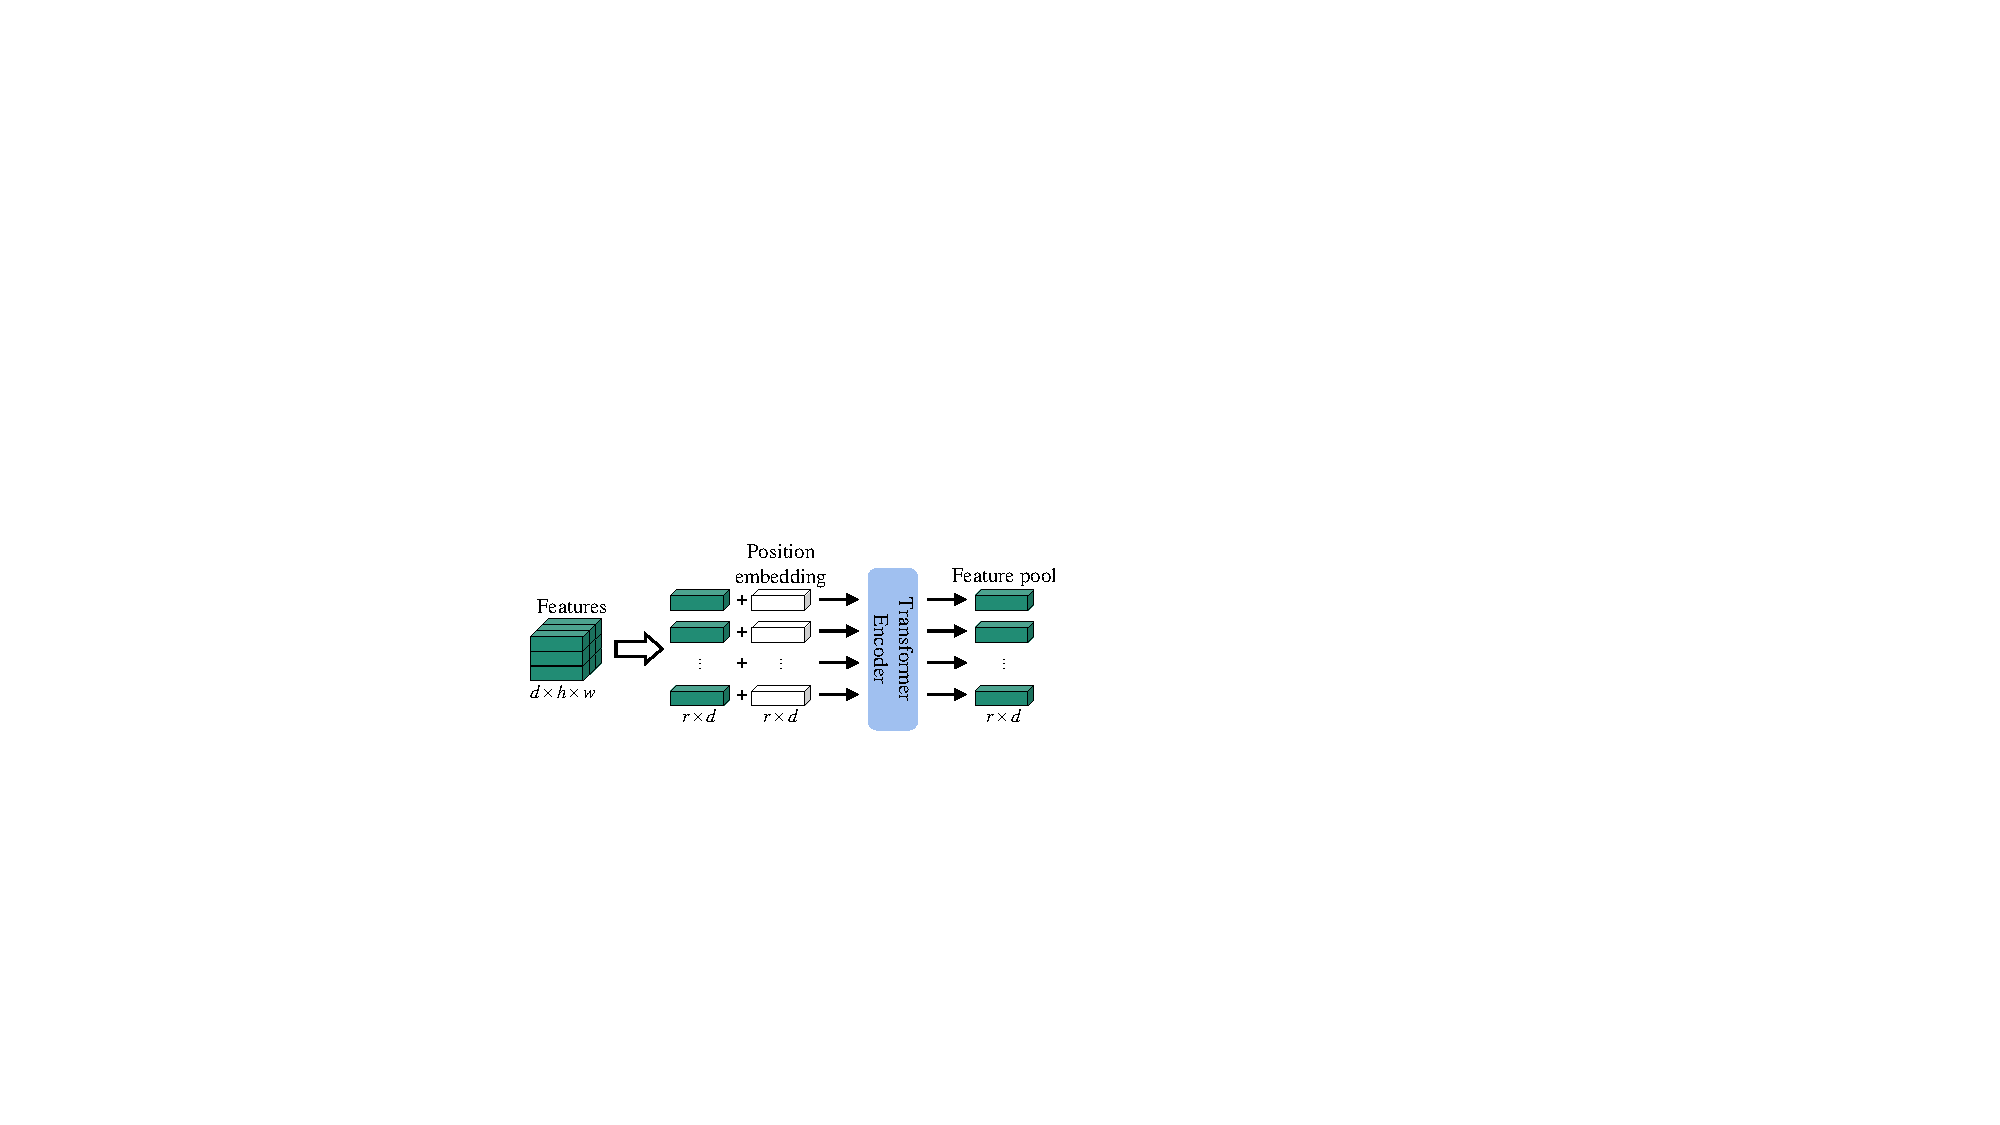
\includegraphics[width=0.85\linewidth]{figures/3.2.pdf}
  \caption{Feature self-reconstruction module.}
  \label{fig:3.2}
\end{figure}

We constructed the feature self-reconstruction module (FSRM), as shown in Figure~\ref{fig:3.2}. For a $C$-way $K$-shot classification task, we input $C \times (K+M)$ samples $x_i$ into the embedding module $f_{\theta}$ to extract features $\hat{x_i} = f_\theta(x_i) \in \mathbb{R}^{d\times h \times w}$, where $d$ is the channel number, $h$ and $w$ represents the height and the width of features, respectively.
Each image feature $\hat{x_i}$ is the input of the FSRM, $g_{\phi}$, and the output of the FSRM is recorded as ${\hat{z_i}} \in \mathbb{R}^{r \times d}$.

First, we reshape the feature $\hat{x_i}$ as $r$ local features in spatial positions $[\hat{x}_i^1, \hat{x}_i^2, \cdots, \hat{x}_i^{r}]$, where $r=h\times w$. The traditional vision transformers~\cite{dosovitskiy2021an} build on standard transformers~\cite{NIPS2017_3f5ee243}, taking the sequence of image patches as input. We {however} compute the summation of the sequence of local features $\hat{x}_i^{j}$ and the corresponding spatial position embedding $E_{pos} \in R^{r \times d}$ as the input of the transformer, i.e.,
  ${z_i} = [\hat{x}_i^1, \hat{x}_i^2, \cdots, \hat{x}_i^{r}] + E_{pos}$,
where $E_{pos}$ adopts sinusoidal position encoding~\cite{NIPS2017_3f5ee243}.

The output of FSRM module is computed based on the standard self-attention operation in Transformer Encoder, and the computing operation is shown as follows:
\begin{equation}
  Attention(Q, K, V) = Softmax(\frac{QK^T}{\sqrt{d_k}})V.
  \label{equ:2}
\end{equation}
Therefore, we can obtain $\hat{z_i}$ as,
\begin{equation}
  \hat{z_i} = Attention(z_i W_{\phi}^Q, z_i W_{\phi}^K, z_i W_{\phi}^V), \hat{z_i} \in \mathbb{R}^{r\times d},
\end{equation}
where $W_{\phi}^Q$, $W_{\phi}^K$, and $W_{\phi}^V$ are a set of learnable weight parameters with $d\times d$ size. Next, the $\hat{z_i}$ are calculated continually by a Layer Normalization ($LN$) and a Multi-Layer Perceptron ($MLP$).
\begin{equation}
  \hat{z_i} = MLP(LN(z_i + \hat{z_i})).
\end{equation}

\subsection{Feature Mutual Reconstruction Module (FMRM)}
\begin{figure}[ht]
  \centering
  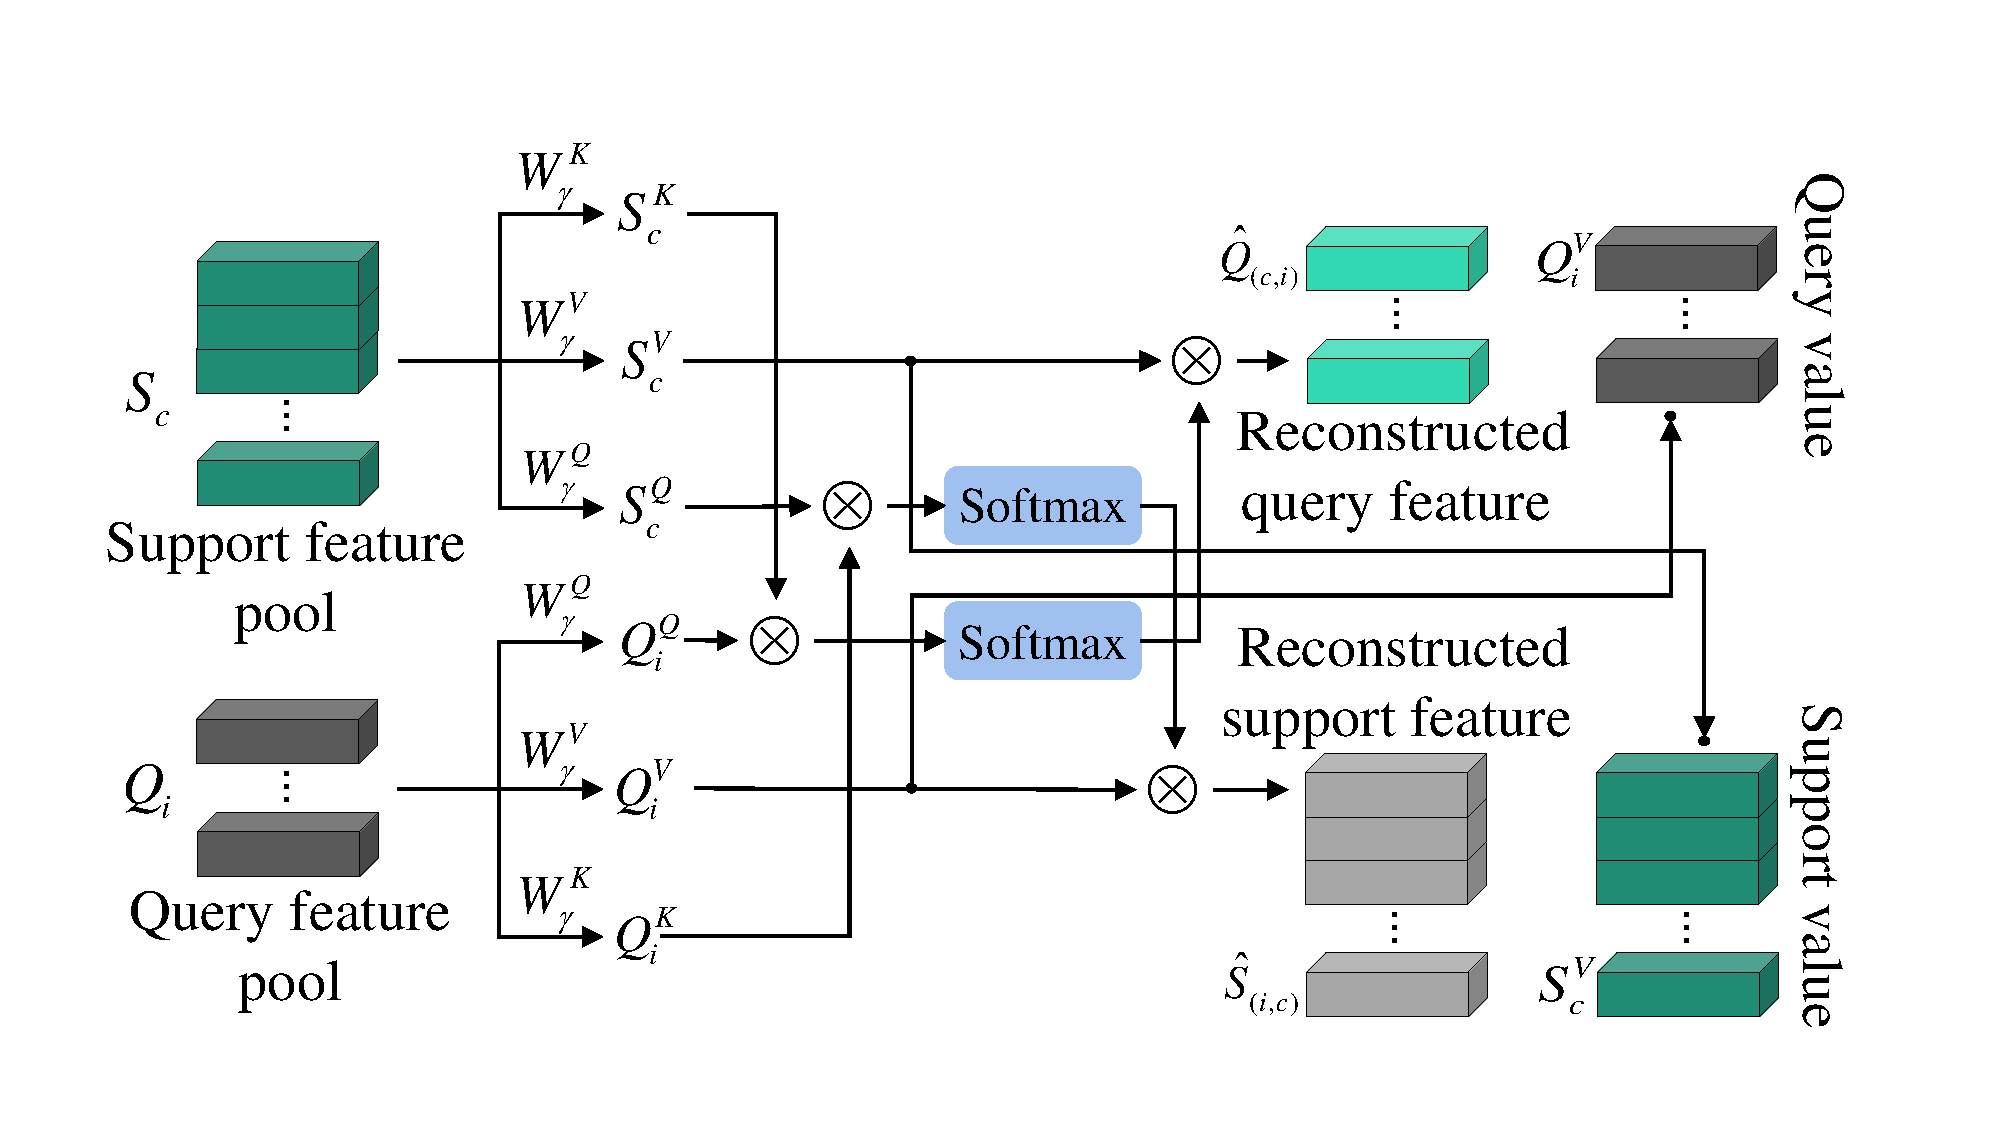
\includegraphics[width=0.8\linewidth]{figures/3.3.pdf}
  \caption{Feature mutual reconstruction module.}
  \label{fig:3.3}
\end{figure}







We propose Feature Mutual Reconstruction Module (FMRM), as shown in Figure~\ref{fig:3.3}, which contains two operations:
reconstructing support features in one class given a query feature and reconstructing query feature given support features in one class.



For $C$-way $K$-shot classification task, after going through FSRM, we can obtain reconstructed support features of the $c^\text{th}$ class, i.e. $S_c = [\hat{z}_k^c] \in \mathbb{R}^{kr\times d} $, where $k \in [1,\cdots, K]$ {and $c \in [1,\cdots, C]$}, and reconstructed query feature $Q_i =\hat{z_i} \in \mathbb{R}^{r\times d}$, where
$i \in [1,\cdots, C\times M]$.
$S_c$ multiplies by weights $W_{\gamma}^Q$, $W_{\gamma}^K$ and $W_{\gamma}^V$,respectively, obtaining $S_c^Q$, $S_c^K$ and $S_c^V$, where $W_{\gamma}^Q, W_{\gamma}^K, W_{\gamma}^V \in \mathbb{R}^{d\times d}$. Similarly, $Q_i$ multiplies by weights $W_{\gamma}^Q$, $W_{\gamma}^K$ and $W_{\gamma}^V$, respectively, obtaining $Q_i^Q$, $Q_i^K$ and $Q_i^V$.








We calculate the reconstructed $i^\text{th}$ query feature $\hat{Q}_{(c,i)}$ from {support features $S_c^V$ in the $c^\text{th}$ class and the reconstructed support features $\hat{S}_{(i,c)}$ in the $c^\text{th}$ class} from $i^\text{th}$ query using the two equations below.



\begin{equation}
\hat{Q}_{(c, i)} = Attention(Q_i^Q, S_c^K, S_c^V), \hat{Q}_{(c, i)} \in \mathbb{R}^{r\times d},
\label{equ:5}
\end{equation}

\begin{equation}
\hat{S}_{(i, c)} = Attention(S_c^Q, Q_i^K, Q_i^V), \hat{S}_{(i, c)}\in \mathbb{R}^{kr\times d}.
\label{equ:6}
\end{equation}
where $Attention(\cdot, \cdot, \cdot)$ is shown in Equation~\ref{equ:2}.

To our best knowledge, the existing reconstruction methods only use unidirectional reconstruction -- using support features to reconstruct the query feature. Building on existing methods, we add the reverse reconstruction shown in Equation~\ref{equ:6} -- using query feature to reconstruct support features.

\subsection{Learning Objectives}



After FMRM, we use the {Euclidean} metric to compute the distance from this query sample $Q_i$ to the support samples in the $c^\text{th}$ class (Figure~\ref{fig:1.2}(b)) as:
\begin{equation}
d_{Q_i \to S_c} = ||Q_i^V - \hat{Q}_{(c, i)}||^2,
\label{equ:7}
\end{equation}
and compute the distance from the support samples in the $c^\text{th}$ class to the query sample $Q_i$ (Figure~\ref{fig:1.2}(c)) as:
\begin{equation}
d_{S_c \to Q_i} = ||S_c^V - \hat{S}_{(i, c)}||^2.
\label{equ:8}
\end{equation}
The total distance can be obtained by weighted summation of two distances $d_{Q_i \to S_c}$ and $d_{S_c \to Q_i}$, as,
\begin{equation}
d_i^c = \tau(\lambda_1 d_{Q_i \to S_c} + \lambda_2 d_{S_c \to Q_i}),
\label{equ:9}
\end{equation}
where $\lambda_1$ and $\lambda_2$ are learnable weight parameters, and both of them are initialized as $0.5$. $\tau$ is a learnable temperature factor, following~\cite{Wertheimer_2021_CVPR, Ye_2020_CVPR, Chen2020ANM, Gidaris2018DynamicFV}.
% \textcolor{red}{The convergence values of $\lambda_1$, $\lambda_2$ and $\tau$ and the effect of different values of $\lambda_1$ and $\lambda_2$ on performance can be found in the supplementary material.}
We normalize $d_i^c$ to obtain $\hat{d_i^c}$ as:
\begin{equation}
\hat{d_i^c} = \frac{e^{-d_i^c}}{\sum_{c=1}^C e^{-d_i^c}}.
\end{equation}
Based on $\hat{d_i^c}$, the total loss in one $C$-way $K$-shot task can be calculated as:
\begin{equation}
\mathcal{L} = -\frac{1}{M \times C} \sum_{i=1}^{M \times C} \sum_{c=1}^C \textbf{1}(y_ i==c) log(\hat{d_i^c}),
\end{equation}
where $\textbf{1}(y_i==c)$ equals $1$ when $y_i$ and $c$ are equal, otherwise $0$.

During the training process, for a $C$-way $K$-shot task on $D_{base}$, we minimize $\mathcal{L}$ to update the proposed network, and repeat this process on all randomly generated tasks.


% \color{red}
% \subsection{In-depth Analysis about the Proposed Mutual Reconstruction}

% We first conjecture that the main challenge for fine-grained few-shot image classification is to learn feature representations with higher inter-class and lower intra-class variations, with just a few labelled samples. This unique combination of limited sample size and fine-grained learning essentially rendered conventional few-shot learning methods incompatible. Prior works predominately use a support set to reconstruct the query image and then utilize metric learning to form fine-grained learning. Upon careful inspection, we importantly reveal that the problem essentially comes down to the inability of existing unidirectional models on minimising intra-class variations. Contrarily, our model tackles this by increasing inter-class variations while reducing intra-class variations mainly via the Feature Mutual Reconstruction Module (FMRM).

% Concretely speaking, given the total distance $d_i^c$ between a query sample $Q_i \in \mathbb{R}^{r\times d}$ and a support class $S_c$ ($c \in [1,\cdots, C]$) as:
% \begin{equation}
% d_i^c = \tau(\lambda_1 d_{Q_i \to S_c} + \lambda_2 d_{S_c \to Q_i})
% \label{equ:9}
% \end{equation}


% \begin{equation}
% \begin{aligned}
%     & d_{Q_i \to S_{c}} = & \\
%     & ||Q_i W_{\gamma}^V - \sigma(\frac{Q_i W_{\gamma}^Q (\mathop{||} \limits_{k=1}^K{(S_{(c,k)} W_{\gamma}^K})^T} {\sqrt{d}}) \mathop{{||}} \limits_{k=1}^K (S_{(c,k)} W_{\gamma}^V )||^2 &\\
% \end{aligned}
% \end{equation}




% \begin{equation}
% \begin{aligned}
%     & d_{S_{c} \to Q_i}  = \\
%     & ||\mathop{{||}} \limits_{k=1}^K
%         (S_{(c,k)} W_{\gamma}^V ) -
%          \sigma(\frac{\mathop{{||}} \limits_{k=1}^K( S_{(c,k)} W_{\gamma}^Q )(Q_i W_{\gamma}^K)^T}{\sqrt{d}}) Q_i W_{\gamma}^V||^2
% \end{aligned}
% \end{equation}
% , where $d_{Q_i \to S_c}$ is the distance from this query sample $Q_i$ to the support samples in the $c^\text{th}$ class (i.e., reconstructing query samples based on support samples), and $d_{S_c \to Q_i}$ on the contrary represents the distance from the support samples in the $c^\text{th}$ class to the query sample $Q_i$ (i.e., reconstructing support samples based on the query sample). Here, $W_{\gamma}^Q, W_{\gamma}^K, W_{\gamma}^V \in \mathbb{R}^{d\times d}$ are the three parameter matrices in FMRM, $S_{(c,k)} \in \mathbb{R}^{r\times d}$ represents the $k$th support sample feature in the $c$th class, and $||$ represents the concatenation operation along the row dimension of a matrix.

% Assuming $W_{\gamma}^Q=I, W_{\gamma}^V =I$ for simplicity, we have
% \begin{equation}
% \begin{aligned}
%     d_{Q_i \to S_{c}} =
%     ||Q_i- \sigma(\frac{Q_i\mathop{{||}} \limits_{k=1}^K({S_{(c,k)} W_{\gamma}^K})^T} {\sqrt{d}})  \mathop{{||}} \limits_{k=1}^K S_{(c,k)}||^2
% \end{aligned}\label{Equ:QtoS}
% \end{equation}


% From this, we can conclude that during the classification operation of $d_{Q_i \to S_{c}}$, the optimization objective must satisfy $\forall \; Q_i$, $d_{Q_i \to S_{c}} \ll d_{Q_i \to S_{t}} $, where $c$ is the corresponding label of $Q_i$, $t,c\in [1,\cdots, C]$, and $t\neq c$. This means, that only the $c^\text{th}$ support class $\mathop{{||}} \limits_{k=1}^K S_{(c,k)}$ can act as the reconstruction pool of $Q_i$. Other support classes do not contain {enough} elements needed to reconstruct $Q_i$. To this end, we can say that $d_{Q_i\to S_c}$ is responsible for increasing inter-class variations.

% Likewise for $d_{S_{c} \to Q_i}$, we have:
% \begin{equation}
% \begin{aligned}
%     d_{S_{c} \to Q_i}
%     = \sum_{k=1}^K|| S_{(c,k)}-\sigma(\frac{S_{(c,k)}  (Q_i W_{\gamma}^K)^T}{\sqrt{d}}) Q_i||^2 \\
% \end{aligned}
% \label{Equ:StoQ}
% \end{equation}
% Again, we can conclude that the optimization objective for $d_{S_{c} \to Q_i}$ also must satisfy $\forall \; Q_i$ and its label $c$, $d_{Q_i \to S_{c}} \ll d_{Q_i \to S_{t}} $, where $t\in [1,\cdots, C]$, and $t\neq c$, and that each support feature $S_{(c,k)}$, $k\in [1,\cdots, K]$, can be reconstructed by $Q_i$.

% So, for the ideal case of $d_{S_{c} \to Q_i} =0$, for any two support sample $S_{(c,h)}$ and $S_{(c,j)}$ in the $c$th class, we have
% \begin{equation}
% \begin{aligned}
%      ||S_{(c,h)}-S_{(c,j)} ||^2 & =||\sigma(\frac{S_{(c,h)}  (Q_i W_{\gamma}^K)^T}{\sqrt{d}}) Q_i \\
%      & \quad -\sigma(\frac{S_{(c,j)}  (Q_i W_{\gamma}^K)^T}{\sqrt{d}})Q_i||^2 \\
%     &\leq 2 r||Q_i||^2 \\
% \end{aligned}
% \end{equation}


% Similarly we can conclude $d_{S_{c} \to Q_i}$ to be responsible for reducing intra-class variations.
% Now, for existing unidirectional models, the second guiding signal of $d_{S_{c} \to Q_i}$ is missing, thus leaving large intra-class variations unattended.
% On the contrary, our model having both ($d_{Q_i\to S_c}$ and $d_{S_{c} \to Q_i}$), performs bi-directional reconstruction between both support and query samples, thus reducing intra-class variations besides increasing inter-class variations.
% \color{black}




\section{Experimental results and Analysis}




\subsection{Datasets and Implementation Details}\label{data_imp}
\textbf{Datasets:}
To evaluate the performance of the proposed method, we selected {three} benchmark fine-grained datasets,
CUB-200-2011 (CUB)~\cite{WelinderEtal2010} is a classic fine-grained image classification dataset. It contains $11,788$ images from $200$ bird species. Following~\cite{Zhang_2020_CVPR,Ye_2020_CVPR}, we crop each image to a human annotated bounding box.
Stanford-Dogs (Dogs)~\cite{KhoslaYaoJayadevaprakashFeiFei_FGVC2011} is a challenging fine-grained image categorization dataset. The dataset includes $20,580$ annotated images of $120$ breeds of dogs from around the world.
Stanford-Cars (Cars)~\cite{6755945} is also a commonly used benchmark dataset for fine-grained image classification. The dataset contains $16,185$ images of $196$ car-types.
For each dataset, we divided it into $D_{train}$, $D_{val}$ and $D_{test}$. The ratio of $D_{train}$, $D_{val}$ and $D_{test}$ is same as the literature ~\cite{zhu2020multi}, and all images are resized to $84 \times 84$.







\textbf{Implementation Details:}
{We conducted experiments on two widely used backbone architectures: Conv-4 and ResNet-12. The architectures of Conv-4 and ResNet-12 are the same as that of ~\cite{Wertheimer_2021_CVPR, Ye_2020_CVPR}.
We implemented all our experiments on NVIDIA 3090Ti GPUs via Pytorch~\cite{Paszke2019PyTorchAI}.
In our experiments, we train all Conv-4 and ResNet-12 models for $1,200$ epochs using SGD with Nesterov momentum of $0.9$. The initial learning rate is set to $0.1$ and weight decay to 5e-4. Learning rate is decreased by a scaling factor of 10 after every 400 epochs.
For Conv-4 models, we train the proposed models using $30$-way $5$-shot episodes, and test for $1$-shot and $5$-shot episodes. We use $15$ query images per class in both settings.
Furthermore, for ResNet-12 models we train our proposed model using $15$-way $5$-shot episodes, in order to save memory.
We employ standard data augmentation, including center crop, random horizontal flip and colour jitter for better training stability. Thereafter, we select the best-performing model based on the validation set, and validate every $20$ epochs. For all experiments, we report the mean accuracy of $10,000$ randomly generated tasks on $D_{test}$ with $95\%$ confidence intervals on the standard $5$-way, $1$-shot and $5$-shot settings.}








\subsection{Comparison with State-of-the-Arts}
\begin{table*}[!ht]
\setlength\tabcolsep{4.8pt}
\centering
\caption{5-way few-shot classification performance on the \textit{CUB}, \textit{Dogs} and \textit{Cars} datasets. {The top block uses Conv-4 backbone and the bottom block uses ResNet-12 backbone.} Methods labeled by $\dag$ denote our implementations.}
\label{tab:1}
\begin{tabular}{ccccccc}
\toprule[1pt]
\multirow{2}{*}{\it{Method}}
& \multicolumn{2}{c}{\it{CUB}}
& \multicolumn{2}{c}{\it{Dogs}}
& \multicolumn{2}{c}{\it{Cars}}  \\

&\multicolumn{1}{c}{$1$-shot}
& \multicolumn{1}{c}{$5$-shot}
& \multicolumn{1}{c}{$1$-shot}
& \multicolumn{1}{c}{$5$-shot}
& \multicolumn{1}{c}{$1$-shot}
& \multicolumn{1}{c}{$5$-shot} \\ \midrule


ProtoNet$\dag$~(NeurIPS 2017)%\cite{NIPS2017_cb8da676}
& 64.82$\pm$0.23
& 85.74$\pm$0.14
& 46.66$\pm$0.21
& 70.77$\pm$0.16
& 50.88$\pm$0.23
& 74.89$\pm$0.18 \\

Relation~(CVPR 2018)%\cite{8578229}
& 63.94$\pm$0.92
& 77.87$\pm$0.64
& 47.35$\pm$0.88
& 66.20$\pm$0.74
& 46.04$\pm$0.91
& 68.52$\pm$0.78 \\

DN4~(CVPR 2019)%\cite{8953758}
& 57.45$\pm$0.89
& 84.41$\pm$0.58
& 39.08$\pm$0.76
& 69.81$\pm$0.69
& 34.12$\pm$0.68
& {87.47$\pm$0.47} \\



PARN$\dag$~(ICCV 2019)%\cite{Wu_2019_ICCV}
& {74.43$\pm$0.95}
& 83.11$\pm$0.67
& 55.86$\pm$0.97
& 68.06$\pm$0.72
& 66.01$\pm$0.94
& 73.74$\pm$0.70 \\


SAML~(ICCV 2019)%\cite{Hao2019CollectAS}
& {65.35$\pm$0.65}
& 78.47$\pm$0.41
& 45.46$\pm$0.36
& 59.65$\pm$0.51
& 61.07$\pm$0.47
& 88.73$\pm$0.49 \\

DeepEMD~(CVPR 2020)%\cite{Zhang_2020_CVPR}
& 64.08$\pm$0.50
& 80.55$\pm$0.71
& 46.73$\pm$0.49
& 65.74$\pm$0.63
& 61.63$\pm$0.27
& 72.95$\pm$0.38 \\


LRPABN~(TMM 2021)%\cite{Huang2021LowRankPA}
& 63.63$\pm$0.77
& 76.06$\pm$0.58
& 45.72$\pm$0.75
& 60.94$\pm$0.66
& 60.28$\pm$0.76
& 73.29$\pm$0.58 \\


BSNet(D\&C)~(TIP 2021)%\cite{9293172}
& 62.84$\pm$0.95
& 85.39$\pm$0.56
& 43.42$\pm$0.86
& 71.90$\pm$0.68
& 40.89$\pm$0.77
& 86.88$\pm$0.50 \\

CTX$\dag$~(NeurrIPS 2020)%\cite{NEURIPS2020_fa28c6cd}
& 72.61$\pm$0.21
& 86.23$\pm$0.14
& 57.86$\pm$0.21
& 73.59$\pm$0.16
& 66.35$\pm$0.21
& 82.25$\pm$0.14 \\


FRN$\dag$~(CVPR 2021)%~\cite{Wertheimer_2021_CVPR}
& 74.90$\pm$0.21
& 89.39$\pm$0.12
& 60.41$\pm$0.21
& 79.26$\pm$0.15
& 67.48$\pm$0.22
& 87.97$\pm$0.11 \\

FRN+TDM$\dag$~(CVPR 2022)%~\cite{lee2022task}
& 72.01$\pm$0.22
& 89.05$\pm$0.12
& 51.57$\pm$0.23
& 75.25$\pm$0.16
& 65.67$\pm$0.22
& 86.44$\pm$0.12  \\


FRN+TDM (-noise)$\dag$~(CVPR 2022)%~\cite{lee2022task}
& 76.55$\pm$0.21
& 90.33$\pm$0.11
& 62.68$\pm$0.22
& 79.59$\pm$0.15
& 71.16$\pm$0.21
& 89.55$\pm$0.10  \\



Ours
& \textbf{79.08$\pm$0.20}
& \textbf{92.22$\pm$0.10}
& \textbf{64.74$\pm$0.22}
& \textbf{81.29$\pm$0.14}
& \textbf{75.74$\pm$0.20}
& \textbf{91.58$\pm$0.09} \\ \midrule



ProtoNet$\dag$~~(NeurIPS 2017)%\cite{NIPS2017_cb8da676}
& 81.02$\pm$0.20
& 91.93$\pm$0.11
& 73.81$\pm$0.21
& 87.39$\pm$0.12
& 85.46$\pm$0.19
& 95.08$\pm$0.08 \\


CTX$\dag$~(NeurIPS 2020)%\cite{NEURIPS2020_fa28c6cd}
& 80.39$\pm$0.20
& 91.01$\pm$0.11
& 73.22$\pm$0.22
& 85.90$\pm$0.13
& 85.03$\pm$0.19
& 92.63$\pm$0.11 \\



DeepEMD$\dag$~(CVPR 2020)%\cite{Zhang_2020_CVPR}
& 75.59$\pm$0.30
& 88.23$\pm$0.18
& 70.38$\pm$0.30
& 85.24$\pm$0.18
& 80.62$\pm$0.26
& 92.63$\pm$0.13  \\



FRN$\dag$~(CVPR 2021)%\cite{Wertheimer_2021_CVPR}
& 84.30$\pm$0.18
& 93.34$\pm$0.10
& {76.76$\pm$0.21}
& {88.74$\pm$0.12}
& 88.01$\pm$0.17
& 95.75$\pm$0.07 \\

FRN+TDM$\dag$~(CVPR 2022)%\cite{lee2022task}
& 85.15$\pm$0.18
& 93.99$\pm$0.09
& \textbf{78.02$\pm$0.20}
& \textbf{89.85$\pm$0.11}
& 88.92$\pm$0.16
& 96.88$\pm$0.06  \\



FRN+TDM (-noise)$\dag$~(CVPR 2022)%\cite{lee2022task}
& 84.97$\pm$0.18
& 93.83$\pm$0.09
& 77.94$\pm$0.21
& 89.54$\pm$0.12
& 88.80$\pm$0.16
& 97.02$\pm$0.06  \\

Ours
& \textbf{85.44$\pm$0.18}
& \textbf{94.73$\pm$0.09}
& {76.89$\pm$0.21}
& 88.27$\pm$0.12
& \textbf{90.44$\pm$0.15}
& \textbf{97.49$\pm$0.05} \\ \bottomrule
\end{tabular}
\end{table*}




\begin{table*}[!htp]
\centering
\caption{Ablation studies using only FSRM module or FMRM module.}
\label{tab:3}
\begin{tabular}{ccccccccc}
\toprule[1pt]
  \multirow{2}{*}{\it{Backbone}}
&
\multirow{2}{*}{\it{Method}}
& \multicolumn{2}{c}{\it{CUB}}
& \multicolumn{2}{c}{\it{Dogs}}
& \multicolumn{2}{c}{\it{Cars}} \\

&
& \multicolumn{1}{c}{$1$-shot}
& \multicolumn{1}{c}{$5$-shot}
& \multicolumn{1}{c}{$1$-shot}
& \multicolumn{1}{c}{$5$-shot}
& \multicolumn{1}{c}{$1$-shot}
& \multicolumn{1}{c}{$5$-shot} \\ \midrule

\multirow{4}{*}{Conv-4}
&
Baseline (ProtoNet)
& 64.82$\pm$0.23
& 85.74$\pm$0.14
& 46.66$\pm$0.21
& 70.77$\pm$0.16
& 50.88$\pm$0.23
& 74.89$\pm$0.18 \\

&
(FSRM)
& 75.37$\pm$0.21
& 88.61$\pm$0.12
& \textbf{65.10$\pm$0.22}
& 79.94$\pm$0.15
& 71.61$\pm$0.22
& 84.70$\pm$0.14 \\

&
(FMRM)
& 74.92$\pm$0.21
& 89.97$\pm$0.11
& 61.28$\pm$0.21
& 80.07$\pm$0.14
& 70.22$\pm$0.21
& 88.45$\pm$0.11 \\

&
(FSRM+FMRM)
& \textbf{79.08$\pm$0.20}
& \textbf{92.22$\pm$0.10}
& 64.74$\pm$0.22
& \textbf{81.29$\pm$0.14}
& \textbf{75.74$\pm$0.20}
& \textbf{91.58$\pm$0.09} \\ \midrule


\multirow{4}{*}{ResNet-12}
&
Baseline (ProtoNet)
& 81.02$\pm$0.20
& 91.93$\pm$0.11
& 73.81$\pm$0.21
& 87.39$\pm$0.12
& 85.46$\pm$0.19
& 95.08$\pm$0.08 \\

&
(FSRM)
& 82.53$\pm$0.19
& 92.43$\pm$0.10
& 75.64$\pm$0.21
& 87.44$\pm$0.12
& 85.95$\pm$0.18
& 94.44$\pm$0.08 \\

&
(FMRM)
& 84.33$\pm$0.18
& 94.25$\pm$0.09
& 76.29$\pm$0.21
& \textbf{89.06$\pm$0.11}
& 89.62$\pm$0.15
& 97.45$\pm$0.05 \\

&
(FSRM+FMRM)
& \textbf{85.44$\pm$0.18}
& \textbf{94.73$\pm$0.09}
& \textbf{76.89$\pm$0.21}
& 88.27$\pm$0.12
& \textbf{90.44$\pm$0.15}
& \textbf{97.49$\pm$0.05}  \\ \bottomrule
\end{tabular}
\end{table*}






To validate the efficiency of our method for fine-grained few-shot image classification, we conducted experiments on the {three} fine-grained image classification datasets discussed earlier.
% \textcolor{red}{References for each comparative method can be found in the supplementary material.}
The results of Relation~\cite{8578229}, DN4~\cite{8953758} and BSNet~\cite{9293172} are from literature BSNet~\cite{9293172}, and the results of SAML~\cite{Hao2019CollectAS} and DeepEMD~\cite{Zhang_2020_CVPR} are from DLG~\cite{Cao2022AFF}, and the results of LRPABN~\cite{Huang2021LowRankPA} are from MattML~\cite{zhu2020multi}. The results of methods marked with $\dag$, such as ProtoNet~\cite{NIPS2017_cb8da676}, PARN~\cite{Wu_2019_ICCV}, CTX~\cite{NEURIPS2020_fa28c6cd}, FRN~\cite{Wertheimer_2021_CVPR}, FRN+TDM~\cite{lee2022task} and DeepEMD~\cite{Zhang_2020_CVPR} are obtained via the code officially provided by the author, which is replaced by the dataset used in this paper.


\begin{table*}[!htp]
\centering
\caption{Ablation on reconstruction designs of FMRM.}
\label{tab:4}
\begin{tabular}{cccccccc}
\toprule[1pt]

\multirow{2}{*}{\it{Backbone}}
& \multirow{2}{*}{\it{Method}}
& \multicolumn{2}{c}{\it{CUB}}
& \multicolumn{2}{c}{\it{Dogs}}
& \multicolumn{2}{c}{\it{Cars}} \\

&
& \multicolumn{1}{c}{$1$-shot}
& \multicolumn{1}{c}{$5$-shot}
& \multicolumn{1}{c}{$1$-shot}
& \multicolumn{1}{c}{$5$-shot}
& \multicolumn{1}{c}{$1$-shot}
& \multicolumn{1}{c}{$5$-shot} \\ \midrule

\multirow{4}{*}{Conv-4}
&
Baseline (ProtoNet)
& 64.82$\pm$0.23
& 85.74$\pm$0.14
& 46.66$\pm$0.21
& 70.77$\pm$0.16
& 50.88$\pm$0.23
& 74.89$\pm$0.18 \\

&
Ours (Q$\to$S)
& \textbf{79.88$\pm$0.20}
& 91.76$\pm$0.11
& \textbf{65.26$\pm$0.22}
& 80.81$\pm$0.14
& 75.61$\pm$0.20
& 90.49$\pm$0.10 \\

&
Ours (S$\to$Q)
& 76.54$\pm$0.21
& 88.03$\pm$0.14
& 64.39$\pm$0.22
& 78.36$\pm$0.15
& 72.71$\pm$0.22
& 85.11$\pm$0.14 \\

&
Ours (Mutual)
&  79.08$\pm$0.20
& \textbf{92.22$\pm$0.10}
&  64.74$\pm$0.22
& \textbf{81.29$\pm$0.14}
& \textbf{75.74$\pm$0.20}
& \textbf{91.58$\pm$0.09} \\ \midrule

\multirow{4}{*}{ResNet-12}
&
Baseline (ProtoNet)
& 81.02$\pm$0.20
& 91.93$\pm$0.11
& 73.81$\pm$0.21
& 87.39$\pm$0.12
& 85.46$\pm$0.19
& 95.08$\pm$0.08 \\

&
Ours (Q$\to$S)
& 83.72$\pm$0.19
& 93.31$\pm$0.09
& 76.50$\pm$0.21
& 87.95$\pm$0.12
& 87.37$\pm$0.17
& 95.10$\pm$0.08 \\

&
Ours (S$\to$Q)
& 81.72$\pm$0.19
& 90.83$\pm$0.11
& 75.62$\pm$0.22
& 86.47$\pm$0.13
& 85.90$\pm$0.18
& 93.17$\pm$0.10 \\

&
Ours (Mutual)
& \textbf{85.44$\pm$0.18}
& \textbf{94.73$\pm$0.09}
& \textbf{76.89$\pm$0.21}
& \textbf{88.27$\pm$0.12}
& \textbf{90.44$\pm$0.15}
& \textbf{97.49$\pm$0.05} \\ \bottomrule
\end{tabular}
\end{table*}

\begin{figure*}[ht]
  \centering
  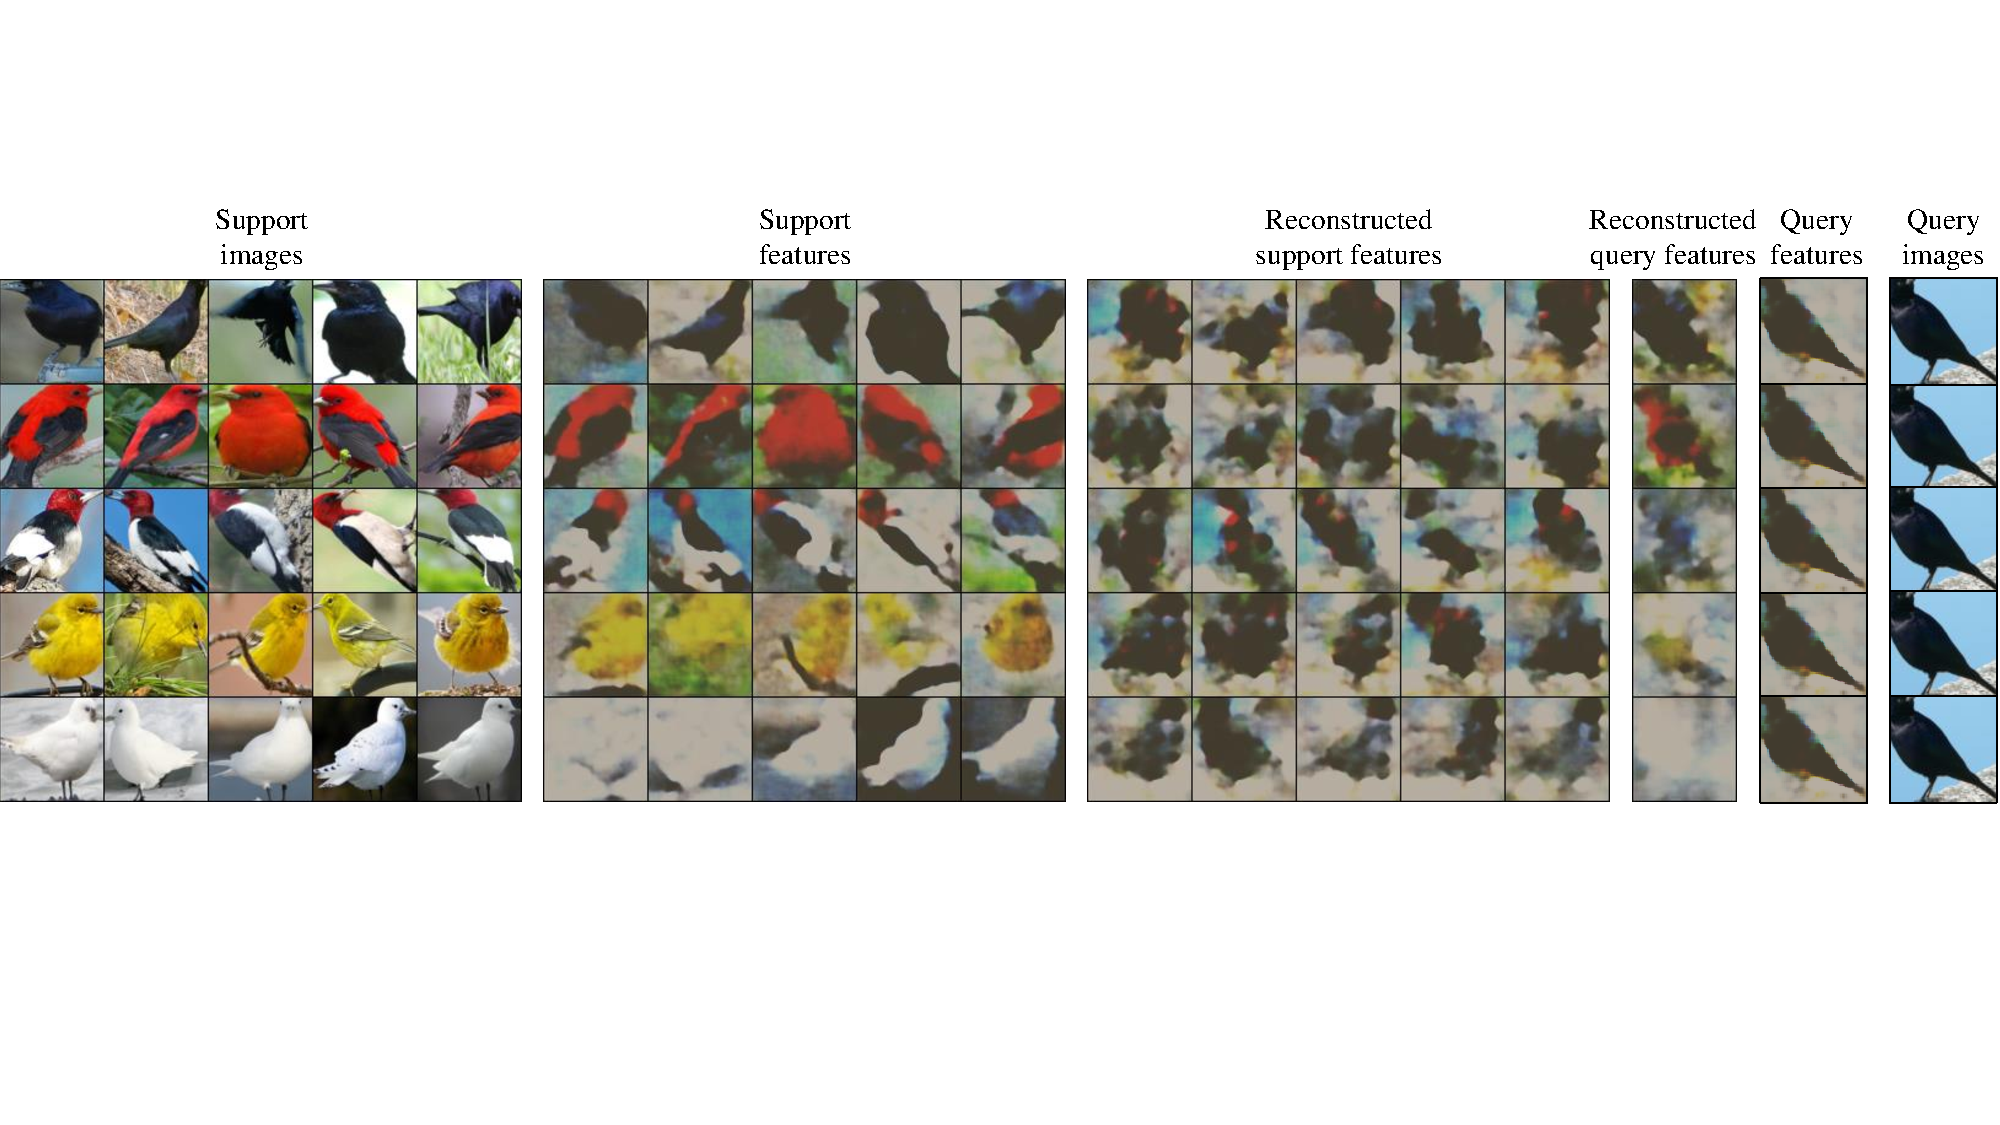
\includegraphics[width=0.8\linewidth]{figures/5.pdf}
  \caption{Recovered images of different features by our method for the CUB dataset. }
  \label{fig:visualize}
\end{figure*}

We use Conv-4 and ResNet-12 as the backbone of all compared methods and test $5$-way $1$-shot and $5$-way $5$-shot classification performance.
As seen from Table~\ref{tab:1}, the proposed method achieves highest accuracy on all three datasets when the Conv-4 is adopted.
Apart from the result on the {Dogs}~\cite{KhoslaYaoJayadevaprakashFeiFei_FGVC2011} dataset where performance falls slightly behind the FRN+TDM method when the ResNet-12 is adopted, our method achieves highest accuracy.


In a nutshell, compared with other newly proposed methods, our method achieves stable and excellent performance on the three fine-grained image datasets on both $5$-way $1$-shot and $5$-way $5$-shot classification tasks, majorly owing to our network structure. The two modules FSRM and FMRM, conditions the model to learn the subtle and discriminative features for fine-grained classification.


\subsection{Ablation Study}\label{Ablation}







To further justify the design choices of our method and model components towards efficiency and accuracy, we perform a few ablation studies on three datasets using both Conv-4 and ResNet-12 as backbone networks.






\textbf{The Effectiveness of FSRM and FMRM:} We compare our method's efficacy by removing components in a strip-down fashion. In other words, we conduct experiments and report in Table~\ref{tab:3}, where we remove FSRM module (\textit{FMRM}), FMRM module (\textit{FSRM}), and then both which becomes equivalent to ProtoNet~\cite{NIPS2017_cb8da676} (\textit{Baseline (ProtoNet)}).
{Evidently, performance improves further in our method where both FSRM and FMRM are used together (\textit{FSRM+FMRM}). Therefore, FSRM and FMRM modules are indispensable and complementary.}



\textbf{The Effectiveness of Mutual Reconstruction in FMRM:}
For our method, we remove reconstruction of support samples based on query samples in FMRM, i.g., $\lambda_2$ becoming $0$ in Equation~\ref{equ:9}, which is marked as Ours ($Q \to S$). And we remove reconstruction of query samples based on support samples, i.g., $\lambda_1$ becoming $0$ in Equation~\ref{equ:9}, which is marked as Ours ($S\to Q$).
{As per Table~\ref{tab:4}, both unidirectional reconstruction methods score lower than the proposed feature mutual reconstruction method (FMRM) in most cases. Therefore, it can be concluded that the design of the Feature Mutual Reconstruction Module (FMRM) is reasonable and effective.}










\subsection{Visualization Analysis}


To demonstrate the efficiency of our proposed network better, we recovered the original and reconstructed features. We trained an inverse ResNet as a decoder, the input of which is the feature value in the mutual reconstruction module, and the output of which is a $3 \times 84 \times 84$ recovered image. In the training process, we use an Adam optimizer with an initial learning rate of $0.01$, set batch size as $200$ and train for $1,000$ epochs, with an L1 loss to measure the prediction error.


As per Figure ~\ref{fig:visualize}, the left-most block shows the support images of $5$ classes, each of which occupies one row and contains $5$ images. The right-most column is a query image, which we copied $5$ times simply for convenient comparison and aesthetics.
The second block from left is the recovered images of support features $S_c^V$, whereas second column from the right is the recovered images of the $i^\text{th}$ query features $Q_i^V$.
The third block from left is the recovered images of reconstructed support feature $\hat{S}_{(i,c)}$ based on $i^\text{th}$ query feature, while that from the right is the recovered images of reconstructed query features $\hat{Q}_{(c,i)}$ based on each $c$ class support feature.

From the first and second {blocks} (first being left-most), it can be seen that the decoder we trained is capable of recovering images from features. For the third {and fourth ones}, it can be seen that if  a query sample is used to reconstruct the support samples which has same class as the query sample, the reconstructed features will be similar to the original support features. However if we use a query sample to reconstruct the support samples which has a class different from the query sample, the reconstructed features will be quite different from the original support features. Likewise, when we use support samples to reconstruct the query samples, similar results are obtained. This indicates that the proposed network can effectively alleviate inaccurate similarity measure of the unaligned fine-grained images.


\section{Conclusion}
\label{Conclusion}
In this paper, we proposed a bi-directional feature reconstruction network for few-shot fine-grained image classification. Our major contribution is a mutual reconstruction module that works in both directions, i.e., support to test and test to support. Compared to the existing reconstruction-based methods, the proposed method can achieve larger inter-class variations and lower the intra-class variations which is crucial to fine-grained learning.
Extensive experiments show that the proposed network can perform well on {three} fine-grained image datasets consistently, competing strongly and at times surpassing contemporary state-of-the-arts.

% \section{Acknowledgments}
% This work was supported in part by Beijing Natural Science Foundation under Grant Z200002, in part by National Natural Science Foundation of China (NSFC) No. 62111530146, 62176110, 61906080, 61922015, U19B2036, 62225601, in part by the Young Doctoral Fund of Education Department of Gansu Province under Grant 2021QB-038, in part by Hong-liu Distinguished Young Talents Foundation of Lanzhou University of Technology, in part by a scholarship from China Scholarship Council (CSC) under Grant CSC No.202006470036, and in part by BUPT Excellent Ph.D. Students Foundation No.CX2020105.


Minus dignissimos eveniet ea ad delectus ipsam voluptas consectetur culpa magni inventore, saepe assumenda impedit dicta nostrum, natus rem voluptate, mollitia quis eaque temporibus dolorem quae perspiciatis, quo consectetur amet esse aperiam illum qui ratione ducimus?Cum nobis quae odio temporibus laudantium tenetur, nobis libero qui mollitia quibusdam quo voluptates, consequatur enim eaque, asperiores fugit similique sapiente possimus?Dolor velit autem, dolores animi possimus mollitia labore, laudantium ipsa quisquam maxime nihil iusto perspiciatis ullam enim vitae repellendus provident, sequi earum sint consectetur minus dolores vitae eius rerum qui cumque.Perferendis deleniti voluptatibus architecto asperiores, aspernatur sunt officiis eligendi optio doloremque sit ab laborum obcaecati nostrum.Dolorem autem provident mollitia numquam id consequatur quas perspiciatis sequi possimus, laudantium nam iure, voluptates totam vel repellendus, nemo officia corporis sunt repudiandae doloremque quidem deleniti eos libero, nam accusamus ut dolorem sit temporibus eum maiores recusandae magni quidem?Omnis veritatis amet dolor dicta, porro obcaecati corporis fugiat harum quaerat consequatur qui modi laborum vitae, possimus tenetur aut minima sequi?Pariatur fugit enim ducimus alias veritatis inventore, quae molestias reprehenderit nisi recusandae cupiditate delectus architecto labore unde excepturi, eius unde exercitationem consequuntur non, perferendis reprehenderit quidem magni necessitatibus corporis pariatur porro ipsam atque vel?Voluptas perspiciatis similique earum velit qui corporis aliquam totam modi rerum cumque, sequi provident blanditiis dolorum libero.Hic rerum exercitationem quisquam sed incidunt assumenda esse, voluptate fugiat nam saepe omnis a veniam voluptates,
\bibliography{reference}

\end{document}